\documentclass[10pt]{IEEEtran}
\IEEEoverridecommandlockouts
% The preceding line is only needed to identify funding in the first footnote. If that is unneeded, please comment it out.
\usepackage{cite}
\usepackage{amsmath,amssymb,amsfonts}
\usepackage{algorithmic}
\usepackage{graphicx}
\usepackage{textcomp}
\usepackage{xcolor}
\usepackage{hyperref}
\usepackage{enumerate}
\usepackage{enumitem}
\usepackage{float}
\setlist[enumerate]{label*=\arabic*.}
\hypersetup{
    colorlinks=true,
    linkcolor=blue,
    filecolor=magenta,      
    urlcolor=cyan,
}
\def\BibTeX{{\rm B\kern-.05em{\sc i\kern-.025em b}\kern-.08em
    T\kern-.1667em\lower.7ex\hbox{E}\kern-.125emX}}
\begin{document}

\title{Survey and Taxonomy of Cyber Anomaly Detection Literature\
}

\author{\IEEEauthorblockN{Wayne R. Havey III}
\IEEEauthorblockA{\textit{UCCS}\\
Colorado Springs, CO \\
whavey@uccs.edu}
}

\maketitle

\begin{abstract}
Detection papers can be categorized by their selection of a few key elements. The environment being monitored for anomalies, the type of anomaly being detected, the data needed to perform the detection, the methods used to perform analysis on that data, and specific tools to implement those methods. Additional surveys, taxonomies, and case studies can still fall under the proposed taxonomy. As far as the author knows there has been no single effort to classify detection papers using all of the above mentioned categories. This paper will provide a more complete classification for which a potential researcher, academic or professional, can use to classify detection literature. This classification can be used as an approach to determine if the researcher has done their due diligence in reading about and potentially even implementing enough strategies to detect the gamut of anomalies. 
\end{abstract}

\section{Introduction}
In an ever increasing cyber landscape just like in any increasing population, the level of crime increases with it. Methods to detect crime vary by type. A detective doesn't use the same methods to track a serial killer as he or she does to track a petty thief. At a higher level, the united states doesn't enlist local police to detect threats to national security. The detective looks for different types of clues, asks different questions of different people, and will enlist different tiers of resources to help track down the suspect. The united states will enlist the CIA or FBI to hunt for national threats. The cyber "detective", should think in a similar fashion. That is; defining their domain, what exactly they are attempting to detect, the information that can be gathered from the susceptible environment, the methods which can be applied to that information in order to detect anomalies, and the resources needed to apply that method. \\
At the highest level this papers goal is to assist the cyber detective; a security researcher, in being able to detect every type of cyber anomaly. Of course just as crime slips through undetected so do cyber anomalies. However just as a nation enlists the support of multiple entities with different skill sets (FBI, CIA, Police, Military, etc.) to attempt to catch every type of criminal, requirements should be defined for detections of as many types of cyber anomalies as possible. \\
To help address this issue this paper puts forth a classification model for detect literature. Using this classification a researcher can organize their reading to ensure all relevant detection topics are covered. Additionally, after enough papers are classified using this model gaps in research should become obvious.\\
The main taxonomy is discussed in depth in later sections and is shown in a logic diagram in figure 1. In order to gratify readers with varying levels of interest in the depth of a detect literature taxonomy, other classification approaches are also presented. All classification approaches presented are congruent with one another and the final main taxonomy can be considered to have been bootstrapped from the others. All classification approaches can be applied by answering a series of questions about the literature.

\section{Quick Classification}
On a quick browse a researcher can answer the following three simple questions regarding the paper being read. 
\begin{itemize}
    \item What is being detected?
    \item What data is needed to perform that detection?
    \item What analysis methods are performed on the data to perform the detection?
\end{itemize}
Answering only these can provide a mechanism for which a researcher may be able to see where there is more or less saturation in the field.

\section{A more Comprehensive Approach}
Breaking the above three questions down further however, will provide greater insight and separate literature further. In addition to the three categories mentioned above I propose two more here. The first is to classify the literature by the environment being addressed, this step should be performed first. The second is to classify the paper by whether or not any specific tool is used to implement the proposed methods. This step should be performed last.\\

\subsection{Questions to ask to assist in classifying the Literature}
\begin{itemize}
    \item Is a specific environment addressed?
        \begin{itemize}
            \item Are multiple environments addressed?\\
            The literature may claim that the detection approaches presented work or even are intended to work in any environment, all environments, or a subset of environment types.
        \end{itemize}
    \item Is a specific type of attack addressed?
    \begin{itemize}
        \item Is only one type of attack addressed?
        \item Are multiple types of attacks addressed?
        \item Does the literature claim to address all anomalies, or anomalies in general?
        \begin{itemize}
            \item Does the literature claim to detect malicious behavior, suspicious behavior, just anomalies, or some combination of these?
        \end{itemize}
    \end{itemize}
    \item Do the authors define the necessary data to collect in order to perform their detection method?
        \begin{itemize}
            \item Do the authors specify different data for the detection of different anomalies?
        \end{itemize}
    \item Are the authors proposing a specific method to perform a detection?\\
    This sub category will be referred to as direct detection because the method itself when successfully deployed results in a detection of the anomaly. 
        \begin{itemize}
            \item Is the method performed in an automated fashion? Or is the paper proposing an automated way to perform a known detection method that was previously manual?
            \begin{itemize}
                \item Is the method based off of a machine learning technique?
                \item Is the method based off of "Honey" or "Canary" technology?
                \item Is the method based off of analytics?\\
            There may of course be some overlap among the above listed categories.
            \end{itemize}
        \end{itemize}
    \item Are the authors proposing something that allows existing methods to perform better?\\
    This sub category will be referred to as support method because the presented information does not result in a direct detection of an anomaly but assists other methods in their performance or effectiveness.
    \begin{itemize}
        \item Do they propose a framework or architecture?
        \item Do they propose a way of organizing the data?
        \item Do they propose a way querying the data?
    \end{itemize}
    \item Are the authors using a specific tool to implement the method of detection.
    \begin{enumerate}
        \item Is the tool the authors own creation? 
        \item If a tool is not specified is it because there is no implementation or because the method could be applied using multiple available tools? It is also possible the tool is irrelevant to the proposed method?
    \end{enumerate}
\end{itemize}
Of course many more sub-criteria may exist that can be used for further refinement but the above list contains the primary factors used to classify detection literature. Some examples of further refinement will be seen later in this paper.\\
The above classification brings the cyber detective closer to a complete taxonomy for effective classification.

\section{Novelty} It is known tht taxonomies already exist individually for most categories presented and in some cases for more than one. However, to the knowledge of the author there has been no single taxonomy put together that encompasses all of them and presents them in an order for which a researcher can follow a logical flow to categorize detection literature.

\section{Usefulness}
 Researchers can classify their papers as well as others in the field. This will help them gain insight into what detection methods are saturated, where gaps are, whether or not a paper has done a good job defining how to implement their proposed method and how well it does at defining exactly what it is trying to detect and how. A fully monitored system(s) should be able to cover every attack type, thus defining every data source and method needed and tools that can assist. 

\section{Environments}
 There can be major differences in detection methodologies based on the type of environment. For example in cyber physical systems, such as the systems managing an electrical grid, there are very specific types of logs and highly tailored attacks. Whereas in a computer network comprising of tens or hundreds of hosts running one of several operating systems there are many types of data to collect, and many attack vectors to be aware of. Some methods may overlap but often times detection literature will specify if their proposed techniques are designed for detection in a specific environment. Agrawal et. al. propose a physics based method for detecting insider threats specifically in cyber physical systems\cite{agrawal2018poster}.
The proposed taxonomy puts forth a separation of detect literature based on the following environment types: General IT systems, cyber physical systems, and embedded systems. An example of a general IT system environment is an enterprise network consisting of many, possibly thousands, of endpoints which run one of several operating systems (Windows, Linux, Mac) as well as networking gear. 

\subsection{Environment Type Sub Classification}
\begin{enumerate}
    \item Is the Environment a general IT environment?
    \item Does the paper specifically call out an operating system type?
    \begin{enumerate}
        \item Windows
        \item Linux
        \item Mac
    \end{enumerate}
    \item Is the environment a Cyber Physical System?
        \begin{enumerate}
            \item Does the paper specifically call out the CPS type?
        \end{enumerate}
    \item Is the environment an embedded system?
        \begin{enumerate}
            \item Is it a mobile device?
            \begin{enumerate}
                    \item Android
                    \item Apple
            \end{enumerate}
        \end{enumerate}
    \item Is the environment a wireless network?
\end{enumerate}

\section{Anomaly Types}
The taxonomy puts forth a proposed subsection for classifying cyber anomaly types based on what was seen the most in surveying the literature. There are already several that exist that can be used for this section of the overall classification. Several surveys have already been written that address this topic. The Mitre "ATT\&CK" (Adversary Tactics Techniques and Cyber Killchain) framework may be appropriately be used here\cite{lazarevic2005intrusion}\cite{mitchell2014survey}\cite{axelsson2000intrusion}. Hansman et. el. propose an attack type taxonomy based attack vectors\cite{hansman2005taxonomy}.
This taxonomy proposes classifying anomaly types as one of five top level categories; Malware, APT, Insider threat, Specific threat, behavior in general. \\
Malware is a top level category because it is unique in that the detection mechanism is focused on determining that there is an executable file in the environment that can start and stop, be hidden, and be moved from system to system. This is different from just Anomaly Type a specific tactic since the encapsulation of the tactic in an executable file is what is being detected. The categorization of malware analysis techniques is out of the scope of this paper, the focus here is the detection of the presence of the malware itself. \\
The APT is a top level category due to its distinct nature of being goal oriented. Additionally APTs often perform their operations over a very long period of time causing the temporality of the data being queried to become an issue.  The uniqueness of APTs lie in the fact that the tactics, techniques, and procedures (TTPs) they use work in conjunction with each other to accomplish a mission over time. The detection of an APT within an environment requires Anomaly Type more than one anomaly and being able to associate those anomalies over time in a way that points to the groups presence due to the relationship between them. \\
Insider threat is a top level category because the detection mechanisms have to recognize malicious intentions within the normal user operations. In many types of detections the events extrapolated from the data themselves can point to malicious intent whereas in an insider threat scenario those events could look completely benign.\\
The specific threat category is for literature that focuses on Anomaly Type a particular anomaly or malicious action. Some examples include, a denial of service attack, SQL injection, or command and control channels. \\
Finally, the literature may not call out specifically what it is Anomaly Type from the above list. In this case it should be explicitly stated or at least possible to infer that it is claiming to do one of two things. Those being; detect some subset of anomalous behavior in general or detect all anomalous behavior thereby encompassing all of the above categories. Some examples of the former being Anomaly Type anomalous behavior just within a specific data source, or behaviour that is anomalous because it occurs during a specific time frame. Additionally, literature classified as Anomaly Type general behavior can be sub classified into Anomaly Type suspicious behavior that requires further analysis or explicitly malicious behavior.

\subsection{Distinctions}
An important note is that APTs can and do use malware in their campaigns. So a paper that is discussing the detection of the malware used by a specific APT without correlating that malware with any other TTPs should still fall under the malware category.\\
Literature classified under the specific threat category may claim to provide a means to detect more than one specific threat however if it claims to detect the associations of these different anomalies with each other and a particular group it should fall under the APT category.

\subsection{Anomaly Type Sub Classification}
\cite{hansman2005taxonomy} \cite{hansman2005taxonomy} 
\begin{enumerate}
    \item Malware\cite{gabriel2009analyzing}\cite{tankard2011advanced}
    \begin{enumerate}
        \item Remote Access Trojans (RAT)\cite{wu2017Anomaly Type}
    \end{enumerate}
    \item APT
    \item Insider Threat\cite{mukherjee1994network}
    \item Specific Threat
    \begin{enumerate}
        \item Denial of Service (DOS) \cite{zargar2013survey}\cite{warrender1999Anomaly Type}\cite{lee1999data}
        \\The literature may even break DOS attacks down further.
        \begin{enumerate} 
            \item Distributed
            \item CPU Exhaust
        \end{enumerate}
        \item Surveillance and Probing \cite{lazarevic2005intrusion}
        \begin{itemize}
            \item Keylogger
        \end{itemize}
        \item Command and Control Channels (C2) \cite{chen2014study}\cite{jasek2013apt}\cite{bhatt2014towards}
        \item Web Based Attacks
        \begin{enumerate}
            \item SQL Injection
            \item Cross Site Scripting
        \end{enumerate}
        \item Embedded Systems Attacks
        \item Zero Days \cite{kotenko2012common}\cite{chen2014study}\cite{jeun2012practical}
        \item Side Channel Attacks
        \item Botnets\cite{singh2014big}\cite{awad2017network}
    \end{enumerate}
    \item Behavior
        \begin{enumerate}
            \item Suspicious
            \item Malicious
            \item Subset
            \item All
        \end{enumerate}
\end{enumerate}

\section{Data to Collect}
Clearly the detection of some anomaly requires there to be some form of information for which it can stand out from. It may be argued that the lack of information can also lead to a detection of some anomaly. In either case detection literature should specify the data that needs to be collected and analyzed in order to perform the proposed detection method. If it is not specified it should be implicit what the source is or if it is necessary to collect all possible data sources. Additionally, it is helpful for the literature to specify the collection mechanisms, storage strategy and, if relevant, the retention period. Data sources can be generally classified as belonging to one of four categories. Those being, host based data sources, network based data sources, application based data sources, and sources external to the computing mechanisms of the environment. Examples of the latter would be things like threat intelligence obtained from the internet, or more obscurely; electromagnetic field fluctuations given off from the internals of a running computer. \\
The categories mentioned can be broken down further in the cases of host, and network based data. For host based data, subcategories can include system calls, logs (which can be sub categorized further), performance counters, or agent based. For network data subcategories can include the raw packets travelling over a network medium, abstracted 'netflow' information (source/destination ports/ips, session duration), and network device logs. \\

\subsection{Other Notes on Data collection}
Ideally the classifiable literature should provide not only the data source to collect from but also the format for which the detect method expects that data to be in. Of course most data types will have a default format but certain tools or methods may require that the format be converted to something more universal like json.\\
Detect literature may not explicitly state the data source to collect. In this case it should be inferred what needs to be collected. That inference could be that all possible data should be collected, that one specific type should be collected that is obvious based on the method, or that one of many different types could be sufficient. In the latter case it could be that there is overlap between different sources. For example there is much overlap between data collected from Windows event logs and the data collected from the Windows Sysmon Agent.\\
Further breakdown of data sources could be in the form of event type distinctions. A detect method may specify a need for one event type or one subset of event types. For example a method for Anomaly Type persistence may require the collection of all windows registry related events.

\subsection{Data Source Collected Sub Classification}
\begin{enumerate}
    \item Host Data\cite{jia2017big}\cite{marchetti2016analysis}
    \begin{itemize}
        \item System calls (syscalls) \cite{warrender1999Anomaly Type}\cite{hofmeyr1998intrusion}
        \item Performance Counters
        \item Event Logs
    \end{itemize}
    \item Network Data
        \begin{itemize}
            \item Network flow \cite{kim2013detection}
            \begin{itemize}
                \item Raw packets
                \item Network flow data
            \end{itemize}
            \item Network Device Logs\cite{horne2002management}
            \begin{itemize}
                \item Routers
                \item Switches
                \item Firewalls
            \end{itemize}
        \end{itemize}
    \item Application Data\cite{giura2012context}\cite{ten2010cybersecurity}
    \\Application Logs is a broad category and encompasses any logging that is provided with software. Below are two special types of application logs worth calling out specifically.
        \begin{enumerate}
            \item Agents\cite{garcia2009anomaly}
            \\Agents are a special type of software that are designed (in the context of this paper) to send security information to a system where specific events can be viewed by an analyst. There may be overlap between agents and the default logging mechanisms on the system but the agent is designed to collect specific information and forward it in a specific format.
            \item Honeypots and Canarys\cite{jasek2013apt}
            \\Honeypots are a special type of detection mechanism used to decieve an attacker typically used in conjunction with Canaries which are designed to immediately alert an analyst upon their access or the access of data around them. Honeypot and canary data may come in various formats although typically in the form of network traffic. It is worth separating them from standard network based data because they provide such a specific function. 
        \end{enumerate}
    How does this model apply to devices such as Internet of Things (IOT) devices and Mobile devices.
\end{enumerate}

\section{Detection Methods}
This is the real meat of cyber anomaly detection literature and so comprises the most critical and easily determined part of the taxonomy. Many of the categories presented here can and have been broken down much further in other surveys. It is recommended that for a deeper classification other surveys are explored in conjunction with what is presented below. With that said, there will be breakdowns of the categories presented here representing the most commonly observed detection strategies in the papers analyzed for this survey.\\
The main classification model for detection methods is as follows. The highest level splits detect literature by whether the proposed method is a direct detection method or a support method. Direct detection is defined here as any method by which an anomaly detection is a direct result of the application of the method. A support method is any method that does not itself result in a detection but instead assists in performing detections in general.\\ 
Direct detections can be sub classified into three categories; machine learning techniques, analytics based techniques, and honey/canary techniques. Some additional sub classifications will be presented below but by no means is it a comprehensive list of attack types. \\
Support methods can be sub classified into the following three categories; data organization, architecture, and query methods or languages. Examples for each will be given below however some additional explanation may be necessary for the support methods. Data organization is a support method for which detection literature may describe means for which store, retain, enrich, filter, an parse data. The cyber detective can see that these actions dont in themselves lead to a detection but instead allow other methods to perform more efficiently. Architecture is a support method classification for which the literature describes the system by which an analyst can perform their detect methods. This may include discussions on the high level components required for a detect system down to specific tools that could be included. Query methods or languages is a support method where the literature discusses ways of querying data which can include a new query language, or strategies such as querying data based on temporality. This is distinct from but integrated with running analytics.

\subsection{Other notes on Detection Methods}
While there is a clear distinction between the three main direct detection categories there can and often is overlap between them. It is plain to see how machine learning could be applied to analytic development. By allowing machine learning to inform what behavior is common in an environment and analytic can be developed to detect if there is uncommon behavior being performed.\\
Similarly, there can be overlap between the support methods described. An obvious example is that a query method or language proposed may require data to be stored or tagged in specific way thus encompassed both the query method and data organization sub categories.\\
An important sub classification that can be applied to all detection methods listed is whether or not the literature is discussing them in terms of automation or a manual process. In other words, do the authors present a means for which the detection or support method can be performed/setup through code?\\
A final categorization that can be made on detection literature is whether or not it discusses the human factor. Cyber anomaly detection is quickly becoming a widely studied subject and there are new methods for detection proposed all the time however, at the end of the day, the decision that something that was detected is actually an anomaly (especially a malicious one) is made by a human. Some literature will discuss how their methods actually performed in terms of the analysts that use it. The literature may discuss the users training level or compare their method between multiple types of users. In the same vein, the literature may go into specifics about the way alerts are shown to a user, or discuss the visualizations of the detections.

\subsection{Detection Method Sub Classification}
\begin{enumerate}
    \item Optionally apply to all: Automation vs Manual.
    \item Direct Detection
        \begin{itemize}
            \item Machine Learning\cite{buczak2016survey}\cite{dua2016data} 
            \begin{itemize}
                \item Training\\
                It has been observed that a large amount of detection literature focusing on machine learning techniques make use of the Darpa data set for training. 
                \item Algorithms
                \begin{itemize}
                    \item Two popular examples among the literature surveyed.
                    \begin{itemize}
                        \item Random Forest \cite{singh2014big}
                        \item K-means\cite{asif2011filtering}\cite{hajamydeen2016unsupervised}
                    \end{itemize}
                \end{itemize}
                \item clustering \cite{asif2011filtering}   
                \item classifying
                \item Regression analysis
            \end{itemize}
            \item Analytics\cite{cardenas2013big}
                \item Attack Graphs\cite{abraham2015predictive}
                \item Algorithms\cite{kim2013detection}
            \item Honey and Canary Technology \cite{jasek2013apt}\cite{saud2015towards}
        \end{itemize}
    \item Support Method
        \begin{itemize}
             \item Data Organization
                \begin{itemize}
                    \item Tagging
                \end{itemize}
                \item Architecture
                \item Query Languages\cite{mukherjee1994network}
                \\ Query languages present an interesting detection mechanism that is heavily related to analytics as they provide a means for them to be created them on the fly. Because of this, their effectivness is likely correlated with the skill and knowledge of the analyst. This may be an interesting research topic.
                \begin{itemize}
                    \item Temporality \cite{abraham2015predictive}\cite{abraham2014cyber}
                \end{itemize}
                \item Behavior definition
                    \begin{itemize}                                  \item White Lists\cite{yen2013beehive}
                    \end{itemize}
        \end{itemize}
\end{enumerate}

\section{Tools}
The final categorization for detection literature is to determine what tools are used in implementing the proposed detection method. This subsection is less important but can still provide some interesting insight. The reason it is less important is because often times it is not applicable. For example, if the detection literature is discussing some novel algorithm the tool by which that algorithm is applied may not be relevant. However, in the aforementioned case, a tool may still have been listed in the testing of that algorithm, and so future research may be done applying the algorithm Tool a different tool or tool set.\\
This categorization level can provide insight into how a particular method can be perform better with a particular tool. In some cases the tool is a primary focus of the literature such as in some examples involving Apache Spark.\\
Similar to other categories the tools listed here are representative of what was most commonly observed in the literature studied for this survey. \\
The sub categorization of tools can be applied by defining whether the tool was one that the authors of the literature created themselves or one they implemented from some other creator(s). If the authors implemented someone else' tool, they should discuss why that one was selected and whether or not they did any comparison with other options. \\
A potential use case for adding this level of classification is to see what methods a tool is not being used for that it potentially could be.

\subsection{Tool Sub Classification}
\begin{enumerate}
    \item Novel
    \item Existing \\
    Some popular examples seen during the survey.
    \begin{itemize}
        \item SIEM \cite{kotenko2012attack}\\
        System Information and Event Management
        \item Weka \cite{asif2011filtering}\cite{thevar2017effect}
        \item Apache Spark \cite{gupta2016framework}\cite{dobson2018performance}
        \item Hadoop \cite{gupta2014big}\cite{tankard2012big}
    \end{itemize}
    \item Commercial \\
    It is important to note that there are commercial detect solutions available and there are often white papers associated with those technologies, which would fall under the umbrella of cyber anomaly detection literature.
\end{enumerate}

\section{The Complete Taxonomy}
Figure 1 shows the complete taxonomy proposed by this survey paper. It can be read similarly to a flowchart diagram. The way to apply it is after or during a read of some form of cyber detection literature perform the following steps. Start at the top left with the "Environment Defined?" decision block. Answer the yes or no question and follow the line for the answer. Each answer will lead to a block that says whether the literature made an explict statement about that particular category, or if you had to infer from context what subcategory to place the literature in. From whichever of those blocks selected, continue following the line to the subcategory box. Determine which subcategory from the list of choices presented in the box the literature falls under. In some cases, particularly in the data source, and detection method categories, there could be multiple that apply. Refer to previous figures for further refinement if there is interest. After applying a subcategory(s) continue to the green dot which will be the start of the dashed line leading to the next main category to classify the literature with. Continue this pattern until reaching the end of the categorization process. It can be seen that for the detection method category the yes or no question is not if the authors define it. This is because if the authors dont define a detection method at all then this taxonomy clearly doesnt apply and the literature doesnt fall under the subfield of cyber anomaly detection literature. Instead what is presented is a yes or no question about the method being a direct detection.\\
For subcategories that often have multiple instances for a single piece of literature, a cycle symbol is placed next to the subcategory box, to denote that you can return to that box multiple times before following the line to the end of the main category section. While only some of subcategories contain the multiple cycle symbol, there can potentially be multiple subcategories applied for any of the sections. However be careful in not over applying. For example if you reach the subcategory box for "anomaly type defined" and you think you can apply the sub category of all of them, then you should just choose APT. This is because, as noted before, APT groups make use of multiple types of attacks.
\begin{figure*}
  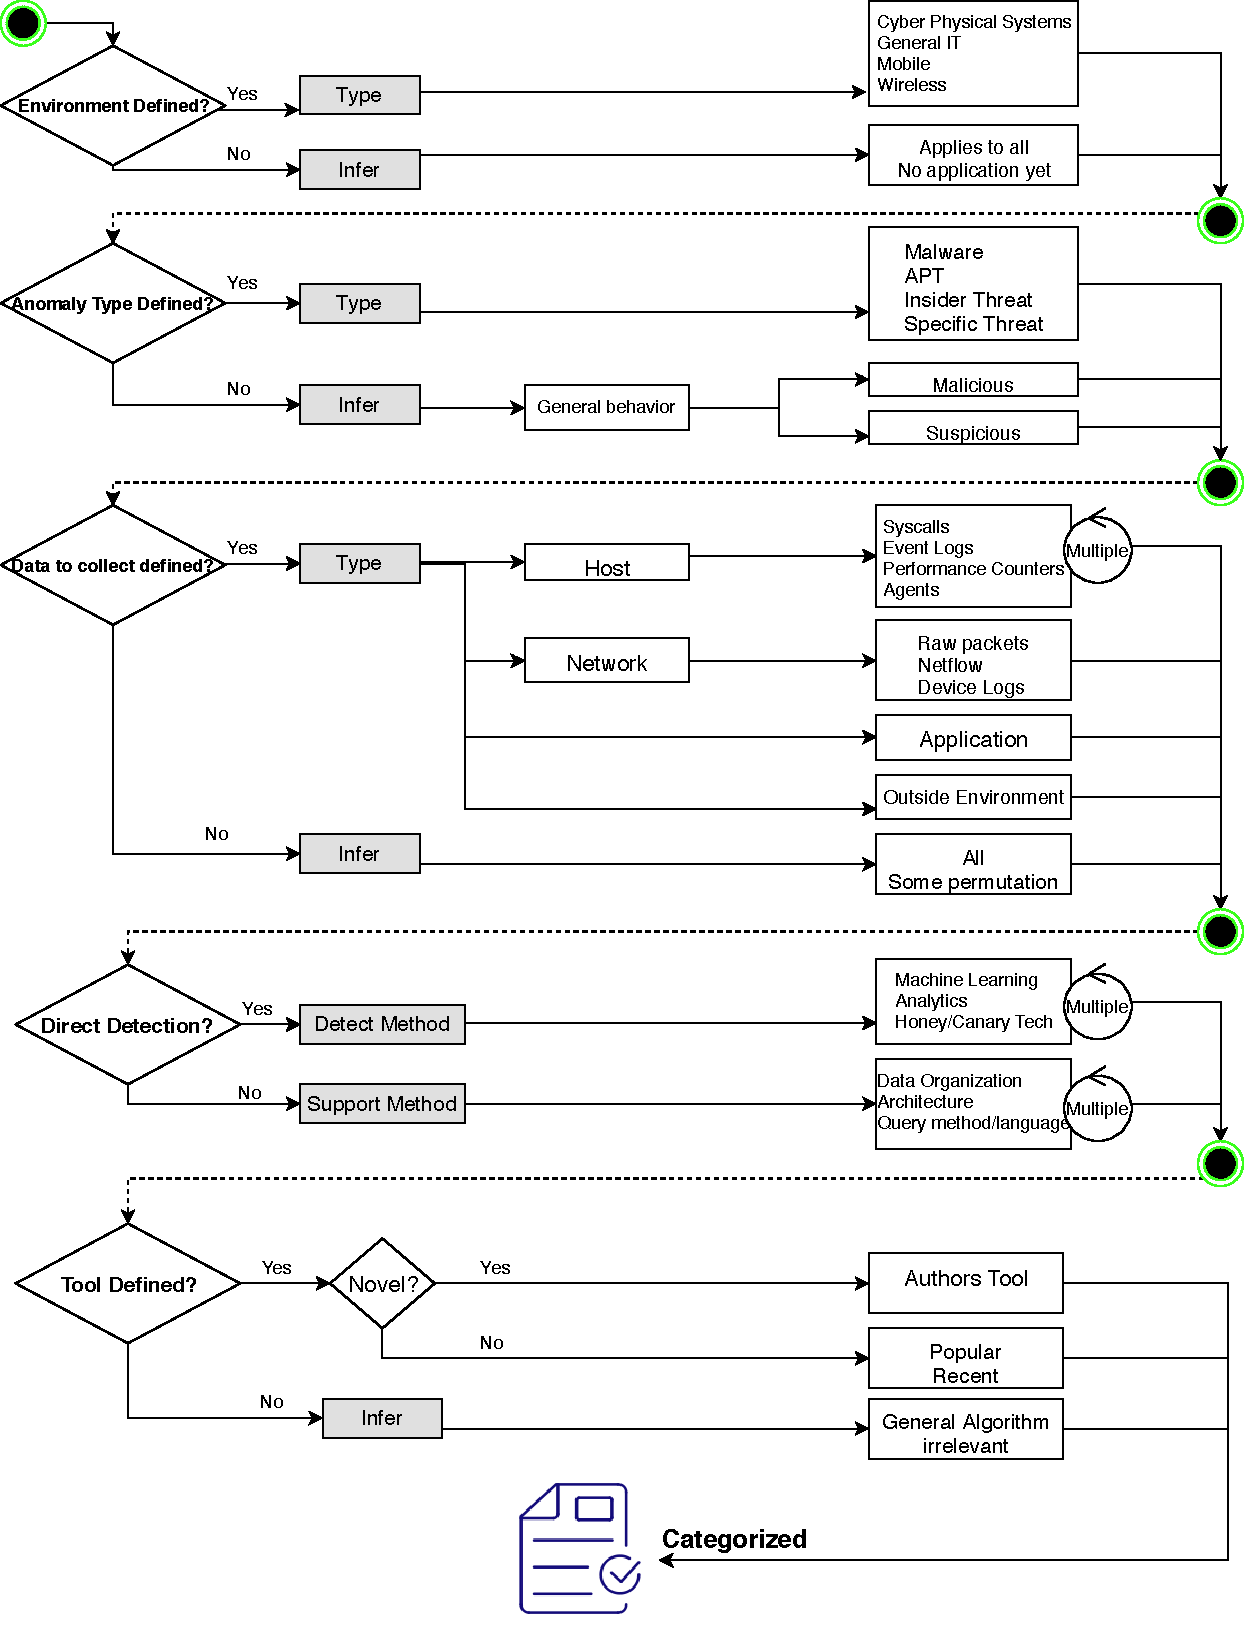
\includegraphics[width=\textwidth]{logicdiagram.pdf}
  \caption{Classification Model}
\end{figure*}

\section{Applications}
\subsection{In Research}
Future researchers could apply the taxonomy to their own literature, and that of literature they cite. This would allow them to produce a figure of a highlighted flow through the taxonomy. Such a figure would allow a reader to quickly determine exactly what the authors are attempting to convey. Additionally, if the authors of future research believe their literature falls somehow outside the confines of this taxonomy, it may be interesting to show where exactly in the process they stand out.\\ Classification of enough literature Tool this taxonomy could reveal where research is lacking, or conversly over-saturated. 

\subsection{In Development and Testing}
This taxonomy could be applied as a testing model, or to define requirements, for a system monitoring platform. When developing such a platform the developers may consult a form of this taxonomy to see if they are creating a system that addresses all potential means of Anomaly Type cyber anomalies. Additionally, they may consult it to define tests for each detection type for the platform.

\section{Potential Future Work}
A future project might entail creating some form of web application that would allow a researcher to classify their own literature as well as literature they are reading and referencing Tool the proposed taxonomy. Ideally such an application would allow other researchers to quickly search based off a selection of subcategories and be provided with a list of literature pertaining to their specific interest. This application would also provide insight as to if the taxonomy is missing anything by allowing a user to submit a "not list" subcategory.

\section{Examples of the Taxonomy Applied}
\begin{enumerate}
    \item 
    Anomaly Type remote access trojans through external control at area network borders\cite{wu2017detecting} \\
    Environment: General IT (inferred) \\
    Anomaly Type: Malware 
    \begin{itemize}
        \item Subcategory: RATs
    \end{itemize}  
    Data source: Network flow data\\ 
    Detection Method: Machine Learning
    \begin{itemize}
        \item Subcategory: Naive Bayes and frequent sequence algorithm
    \end{itemize} 
    Tool: General Algorithm
    
    \item 
    Anomaly Type Intrusions Tool System Calls: Alternative Data Models\cite{warrender1999detecting}\\
    Environment: General IT (inferred)\\
    Anomaly Type: Abnormal behavior \\
    Data Source: Host based 
    \begin{itemize}
        \item system calls
    \end{itemize}
    Detect Method: Machine Learning
    \begin{itemize}
        \item Sequence Time Delay embedding
        \item t-stide
        \item RIPPER
        \item Hidden Markov Model
    \end{itemize} 
    Tool: General Algorithms
    
    \item  
    Anomaly Detection of Web-based Attacks\cite{kruegel2003anomaly}\\
    Environment: General IT (inferred) \\   
    Anomaly Type: Specific Threat 
    \begin{itemize}
        \item Web based attacks
    \end{itemize}
    Data Source: Application
    \begin{itemize}
        \item Web server logs (Apache)
    \end{itemize}
    Detect Method: Machine learning\\
    Tool: General Algorithm
    
    \item 
    The Effect of K-Nearest Neighbors Classifier for Intrusion Detection of Streaming of Net-Flows in the Apache Spark Environment\cite{thevar2017effect} \\
    Environment: General IT (inferred) \\
    Anomaly Type: Specific Threat
    \begin{itemize}
        \item DOS
        \item User to root
        \item remote to local
        \item Probing
    \end{itemize} 
    Data Source: Network Based
    \begin{itemize}
        \item Netflow data (streamed)
    \end{itemize} 
    Detect Method: Machine Learning
    \begin{itemize}
        \item K-Nearest Neighbors
    \end{itemize}[]
    Tool: Apache Spark 
    
    
    \item 
    Detection of Advanced Persistent Threat by Analyzing the Big Data Log\cite{kim2013detection}\\
    Environment: General IT (inferred)\\
    Anomaly Type: APT  \\
    Data Source: Network Based
    \begin{itemize}
        \item Flow data (ingress \& egress points)
    \end{itemize}
    Data Source: Application
    \begin{itemize}
        \item Email logs
    \end{itemize}
    Data Source: Host Based
    \begin{itemize}
        \item Syslog (privilege escalation logs)
    \end{itemize}
    Detect Method: Analytics
    \begin{itemize}
        \item Data analysis algorithm
    \end{itemize}
    Tool: General Algorithm
    
    \item 
    Big-data analysis of multi-source logs for anomaly detection on network-based system\cite{jia2017big}\\
    Environment: General IT \\
    Anomaly Type: General Behavior - Suspicious (stated abnormal)\\ 
    Data Source: Multisource\\ 
    Detect Method: Machine Learning\\ 
    Tool: Apache Spark 
    
    
    \item 
    Robustness of the Markov-chain model for cyber-attack detection\cite{ye2004robustness}\\
    Environment: General IT\\
    Anomaly Type: General Behavior - Suspicious (abnormal) \\
    Data Source: Host Based\\
    \begin{itemize}
        \item Unix-Based Audit data
    \end{itemize}
    Detect Method: Machine Learning \\
    \begin{itemize}
        \item Markov Chain (building normal profile)
    \end{itemize}
    Tool: Algorithms implemented in C++
    
    \item 
    Big Data Analytics framework for Peer-to-Peer Botnet detection using Random Forests\cite{singh2014big}\\
    Environment:General IT (inferred)\\
    Anomaly Type: Specific Threat
    \begin{itemize}
        \item Botnets (p2p)
    \end{itemize}\
    Data Source: Network 
    \begin{itemize}
        \item flow data
    \end{itemize}
    Detect Method: Machine Learning 
    \begin{itemize}
        \item random forest
    \end{itemize}
    Tool: mahout, hadoop, HIVE 
    
    \item 
    Towards insider threat detection using web server logs\cite{myers2009towards}\\
    Environment: General IT \\
    Anomaly Type: Insider threat \\
    Data Source: Application
    \begin{itemize}
        \item Web Server logs
    \end{itemize}
    Detect Method: Analytics (not very in depth)\\ 
    Tool: Not relevant
    
    \item 
    Big data analysis system concept for detecting unknown attacks\cite{ahn2014big}\\
    Environment: General IT \\
    Anomaly Type: APT (Focus on Zero Days) \\
    Data Source: All
    Detect Method: Analytics (not well defined)\\ 
    Tool: Nothing specified
    
    \item 
    On the feasibility of online malware detection with performance counters\cite{demme2013feasibility}\\
    Environment: Mobile\\
    Anomaly Type: Malware \\
    Data Source: Host Based
    \begin{itemize}
        \item Performance Counters
    \end{itemize}
    Detect Method: Machine Learning\\ 
    Tool: General Algorithm
    
    \item 
    Data mining methods for detection of new malicious executables\cite{schultz2001data}\\
    Environment: General IT\\
    Anomaly Type: Malware (Focus on New Windows malware binaries)\\
    Data Source: Outside Environment
    \begin{itemize}
        \item Binary metadata
    \end{itemize}
    Detect Method: Machine Learning
    \begin{itemize}
        \item Classification
    \end{itemize}
    Tool: General Algorithm
    
    \item 
    Anomaly based intrusion detection for network monitoring using a dynamic honeypot.\cite{hieb2004anomaly}\\
    Environment: General IT\\
    Anomaly Type: Specific Threat
    \begin{itemize}
        \item Probing
    \end{itemize}
    Anomaly Type: General Behavior - Suspicious
    Data Source: Network Based
    \begin{itemize}
        \item Netflow Data
    \end{itemize}
    Detect Method: Honey Tech\\ 
    Tool: honeypot/net 
    
    \item 
    Topological Vulnerability Analysis: A Powerful New Approach For Network Attack Prevention, Detection, and Response\cite{jajodia2009topological}\\
    Environment: General IT\\
    Anomaly Type: General Behavior - Malicious \\
    Data Source: Application
    \begin{itemize}
        \item Nessus
    \end{itemize}
    Data Source: Host Based
    Data Source: Network Based
    \begin{itemize}
        \item Network Device Logs
    \end{itemize}
    Detect Method: Vulnerability Analysis and Attack Graph Analysis\\ 
    Tool: Custom
    
    \item 
    SAQL: A Stream-based Query System for Real-Time Abnormal System Behavior Detection\cite{gao2018saql}\\
    Environment: General IT\\
    Anomaly Type: General Behavior - Malicious \\
    Data Source: Multiple source logs (not well defined)\\
    Detect Method: Support Method - Query language\\ 
    Tool: Custom
    
    \item 
    Hardware-Assisted Detection of Malicious Software in Embedded Systems\cite{rahmatian2012hardware}\\
    Environment: Embedded Systems\\
    Anomaly Type: Malicious execution \\
    Data Source: Host Based
    \begin{itemize}
        \item Syscall data
    \end{itemize}
    Detect Method: Support Method 
    \begin{itemize}
        \item Architecture
    \end{itemize}
    Detect Method: Analytics
    Tool: FPGA Design
    
    \item 
    Beehive: large-scale log analysis for detecting suspicious activity in enterprise networks\cite{yen2013beehive}\\
    Environment: General IT\\
    Anomaly Type: General Behavior - Suspicious (specifically states only suspicious)\\
    Data Source: Multisource logs (well defined)\\
    Detect Method: Data organization
    \begin{itemize}
        \item Feature extraction
    \end{itemize}
    Detect Method: Machine learning 
    \begin{itemize}
        \item clustering k-mean
    \end{itemize}
    Tool: SIEM 
    
    \item 
    Zero-day malware detection based on supervised learning algorithms of API call signatures\cite{alazab2011zero}\\
    Environment: General IT\\
    Anomaly Type: Malware
    \begin{itemize}
        \item Zero Days
    \end{itemize}
    Data Source: Host Based
    \begin{itemize}
        \item API Calls
    \end{itemize}
    Detect Method: Machine Learning (supervised learning)  \\
    Tool: Weka
    
    \item
    Security Breaches as PMU Deviation: Detecting and Identifying Security Attacks Using Performance Counters\cite{yuan2011security}\\
    Environment:General IT\\
    Anomaly Type: Specific threat
    \begin{itemize}
        \item Code-injection
        \item return to libc
        \item return oriented programming attacks (very well defined)
    \end{itemize}
    Data Source: Host Based
    \begin{itemize}
        \item Performance Counters (branch miss predictions, instruction TLB (iTLB) misses and L2 cache misses, very well defined) \\
    \end{itemize}
    Detect Method: Analytics (normal behavior) \\
    Tool: Novel tool Eumonia 
   
    
    \item
    Network anomaly detection based on TCM-KNN algorithm\cite{li2007network}\\
    Environment: General IT\\
    Anomaly Type: Specific Threat
    \begin{itemize}
        \item Probes
        \item DoS (Denial of Service)
        \item U2R (User to Root)
        \item R2L (Remote to Local))\\
    \end{itemize}
    Data Source: Network Based
    \begin{itemize}
        \item netflow
    \end{itemize}
    Data Source: Application
    \begin{itemize}
        \item Bro
    \end{itemize}
    Detect Method:  Machine Learning (TCM-KNN)\\
    Tool: Bro
    
    \item
    Real time detection of cache-based side-channel attacks using hardware performance counters\cite{chiappetta2016real}\\
    Environment: General IT\\
    Anomaly Type: Specific Threat
    \begin{itemize}
        \item Cache Based Side Channel Attacks (in title) (flush and reload)
    \end{itemize}
    Data Source: Host Based
    \begin{itemize}
        \item Performance Counters
    \end{itemize}
    Detect Method: Machine Learning (supervised learning) 
    Detect Method: analytics
    Tool: Specified architecture
    
    \item
    A Context-Based Detection Framework for Advanced Persistent Threats\cite{giura2012context}\\
    Environment: General IT\\
    Anomaly Type: APT\\
    Data Source: Specifically states ALL data collectable \\
    Detect Method: Support method
    \begin{itemize}
        \item data organization
    \end{itemize}
    Tool: Not relevant
    
    \item
    Towards proactive detection of advanced persistent threat (APT) attacks using honeypots\cite{saud2015towards}\\
    Environment: General IT\\
    Anomaly Type: APT \\
    Data Source: Network Based
    \begin{itemize}
        \item Netflow data
    \end{itemize}
    Detect Method: Honeypot
    Tool: KFSensor
    
    \item
    A data mining framework for building intrusion detection models\cite{lee1999data}\\
    Environment: General IT\\
    Anomaly Type: Specific Threat
    \begin{itemize}
        \item U2R
        \item R2L
        \item DOS
        \item Probing
    \end{itemize}
    Data Source: Network Based
    \begin{itemize}
        \item Netflow data (temporal)
    \end{itemize}
    Detect Method: Machine Learning  \\
    Tool: Bro
    
    \item
    Towards a Framework to Detect Multi-stage Advanced Persistent Threats Attacks\cite{bhatt2014towards}\\
    Environment: General IT\\
    Anomaly Type:  APT\\
    Data Source:  Multisource log data (not well defined)\\
    Detect Method: Support Method
    \begin{itemize}
        \item Architecture
    \end{itemize}
    Detect Method: Analytics
    Tool: Hadoop
    
    \item
    An unsupervised heterogeneous log-based framework for anomaly detection\cite{hajamydeen2016unsupervised}\\
    Environment: General IT\\
    Anomaly Type: General Behavior (anomalies)\\
    Data Source: States multisource (appears to be mostly netflow data from applications)  \\
    Detect Method: Support method 
    \begin{itemize}
        \item Data Organization
    \end{itemize}
    Detect Method: Machine Learning
    Tool: General Algorithm
    
    \item
    Exploratory security analytics for anomaly detection\cite{pierazzi2016exploratory}\\
    Environment: General IT\\
    Anomaly Type: General Behavior (anomalies)\\
    Data Source: Application
    \begin{itemize}
        \item Alerts\\
        A unique data source among the literature surveyed. This paper proposes a method that uses alerts that could have been generated from any data source as its primary one.
    \end{itemize}
    Detect Method: Support Method
    \begin{itemize}
        \item Temporal Data organization (comparison of multiple)
    \end{itemize}
    Tool: General Approach
    
    \item
    DeepLog: Anomaly Detection and Diagnosis from System Logs through Deep Learning\cite{du2017deeplog}\\
    Environment: General IT\\
    Anomaly Type: General behavior (anomalies)\\
    Data Source: Inferring host based logs (not well defined) \\
    Detect Method: Machine Learning 
    \begin{itemize}
        \item Neural Network
    \end{itemize}
    Tool: General Algorithm
    
    \item
    Attack Detection and Identification in Cyber-Physical Systems\cite{pasqualetti2013attack}\\
    Environment: Cyber Physical Systems\\
    Anomaly Type: Specific Threat
    \begin{itemize}
        \item ROP chaining
    \end{itemize}
    Data Source: Outside Environment
    \begin{itemize}
        \item Binary Data
    \end{itemize}
    Detect Method: Machine Learning
    \begin{itemize}
        \item Markov Chain Model
    \end{itemize}
    Tool: General Framework
    
    \item
    Real-Time Detection of Malware Downloads via Large-Scale URL->File->Machine Graph Mining\cite{rahbarinia2016real}\\
    Environment: General IT\\
    Anomaly Type: Malware
    \begin{itemize}
        \item Download of Malware
    \end{itemize}
    Detect Method: Machine Learning (classification) \\
    Data Source: System and Network level events (not well defined) \\
    Tool: General Approach
\end{enumerate}

\section{Conclusion}
A taxonomy was presented for the classification of cyber anomaly detection literature containing five main categories. Those main categories are; environment definition, anomaly type definition, data source definition, detection type definition, and tool definition. This taxonomy can be applied to assist the cyber detective in determining what a certain piece of literature is trying to convey. Additionally, after enough classifications of the taxonomy, some insight may be made about what subareas are over and under saturated. 
A subset of literature in the field was presented with the taxonomy applied. 

\bibliographystyle{IEEEtran}
\bibliography{survey_bibtex}
\end{document}